\documentclass{beamer}\usepackage[]{graphicx}\usepackage[]{xcolor}
% maxwidth is the original width if it is less than linewidth
% otherwise use linewidth (to make sure the graphics do not exceed the margin)
\makeatletter
\def\maxwidth{ %
  \ifdim\Gin@nat@width>\linewidth
    \linewidth
  \else
    \Gin@nat@width
  \fi
}
\makeatother

\definecolor{fgcolor}{rgb}{0.196, 0.196, 0.196}
\newcommand{\hlnum}[1]{\textcolor[rgb]{0.063,0.58,0.627}{#1}}%
\newcommand{\hlsng}[1]{\textcolor[rgb]{0.063,0.58,0.627}{#1}}%
\newcommand{\hlcom}[1]{\textcolor[rgb]{0.588,0.588,0.588}{#1}}%
\newcommand{\hlopt}[1]{\textcolor[rgb]{0.196,0.196,0.196}{#1}}%
\newcommand{\hldef}[1]{\textcolor[rgb]{0.196,0.196,0.196}{#1}}%
\newcommand{\hlkwa}[1]{\textcolor[rgb]{0.231,0.416,0.784}{#1}}%
\newcommand{\hlkwb}[1]{\textcolor[rgb]{0.627,0,0.314}{#1}}%
\newcommand{\hlkwc}[1]{\textcolor[rgb]{0,0.631,0.314}{#1}}%
\newcommand{\hlkwd}[1]{\textcolor[rgb]{0.78,0.227,0.412}{#1}}%
\let\hlipl\hlkwb

\usepackage{framed}
\makeatletter
\newenvironment{kframe}{%
 \def\at@end@of@kframe{}%
 \ifinner\ifhmode%
  \def\at@end@of@kframe{\end{minipage}}%
  \begin{minipage}{\columnwidth}%
 \fi\fi%
 \def\FrameCommand##1{\hskip\@totalleftmargin \hskip-\fboxsep
 \colorbox{shadecolor}{##1}\hskip-\fboxsep
     % There is no \\@totalrightmargin, so:
     \hskip-\linewidth \hskip-\@totalleftmargin \hskip\columnwidth}%
 \MakeFramed {\advance\hsize-\width
   \@totalleftmargin\z@ \linewidth\hsize
   \@setminipage}}%
 {\par\unskip\endMakeFramed%
 \at@end@of@kframe}
\makeatother

\definecolor{shadecolor}{rgb}{.97, .97, .97}
\definecolor{messagecolor}{rgb}{0, 0, 0}
\definecolor{warningcolor}{rgb}{1, 0, 1}
\definecolor{errorcolor}{rgb}{1, 0, 0}
\newenvironment{knitrout}{}{} % an empty environment to be redefined in TeX

\usepackage{alltt}
\usepackage[english]{babel}
\usepackage{graphbox,graphicx}
\usepackage{url}
\usepackage{amsmath}
\usepackage{pifont}
\usepackage[T1]{fontenc}
\usepackage[font=small,labelfont=bf]{caption}
\usepackage{color}
\usepackage{booktabs}
\fontfamily{verdana}\selectfont
\setlength{\unitlength}{\textwidth}  % measure in textwidths
\setbeamercolor{item}{fg=black}
\setbeamertemplate{itemize items}[triangle] % if you want a ball
\setbeamertemplate{itemize subitem}[triangle] % if you want a circle
\setbeamertemplate{itemize subsubitem}[triangle] % if you want a triangle
\newcommand{\code}[1]{{\texttt{#1}}}

%************ Title & Author ***********************
\title{Running MSE analysis with the a4a platform}
\subtitle{Management Strategies Evaluation with FLR and a4a \\ 25-29 November 2019, Ispra, Italy, }
\IfFileExists{upquote.sty}{\usepackage{upquote}}{}
\begin{document}
\author{Ernesto Jardim \\ \normalfont {\scriptsize \href{mailto:ernesto.jardim@ec.europa.eu}{<ernesto.jardim@ec.europa.eu>}}}
\institute{Joint Research Centre \\ European Commission}


%*******************************************
\begin{frame}
\titlepage


\end{frame}

%*******************************************
\begin{frame}
\frametitle{Fisheries management}

\begin{center}
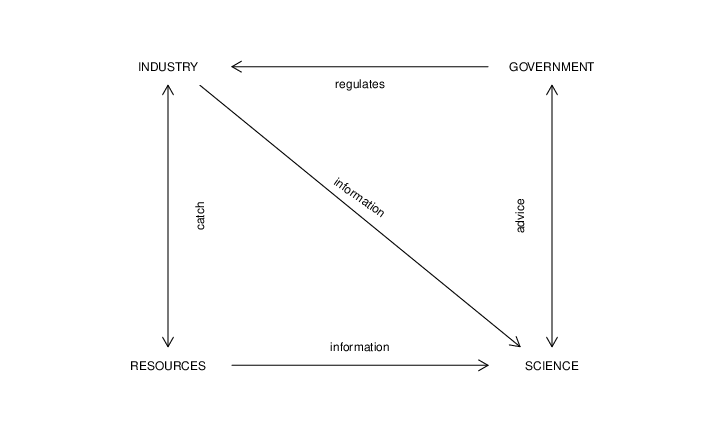
\includegraphics[height=0.95\textheight]{figs/fmanag}
\end{center}

\end{frame}

%*******************************************
\begin{frame}
\frametitle{Goals of fisheries management}

\begin{itemize}
  \item Goals
  \begin{itemize}
    \item Sustainable benefits from harvesting
    \item Conserve stock(s) productivity
    \item Minimise impacts on ecosystem
  \end{itemize}
    \item Requirements
  \begin{itemize}
    \item Set of clear management objectives
    \item Indication of proper harvest and/or stock level
    \item Means to monitor status
    \item Measures to control fishing on advice
  \end{itemize}
\end{itemize}

\end{frame}

%*******************************************
\begin{frame}
\frametitle{Challenges of fisheries management}

\begin{itemize}
  \item Objectives set to be operational
  \item Trade-offs between short and long term
  \item Monitoring impact to ecosystem
  \item Quantifiying uncertainty in status andn dynamics
  \item Making decisions acknowledging risks
\end{itemize}

\end{frame}

%*******************************************
\begin{frame}
\frametitle{How to deal with all this? MSE}

\centering{ \emph{the consequences of a range of different management strategies to determine which one will be the most appropriate to meet the operational objectives of the fishery}}

\begin{itemize}
  \item Goals
  \begin{itemize}
    \item Robustness against uncertainty.
    \item Compare relative performance of alternative MPs.
    \item Simulation-test MPs under a wide(r) range of realities.
  \end{itemize}
\end{itemize}

\end{frame}

%*******************************************
\begin{frame}
\frametitle{Where does this come from?}

- IWC

- New Management Procedure

\begin{center}
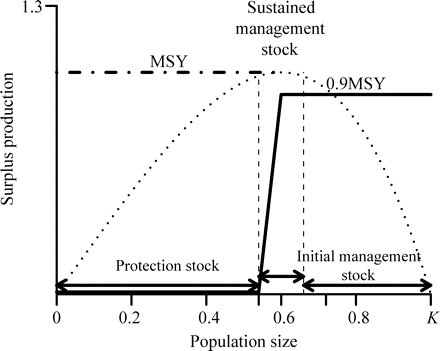
\includegraphics[height=0.4\textheight]{figs/nmp}
\end{center}

- Revised Management Procedure

- Catch Limit Algorithm (CLA)

\end{frame}

%*******************************************
\begin{frame}
\frametitle{IWC: Uncertainties in RMP\footnote{https://iwc.int/rmp2, https://doi.org/10.1093/icesjms/fsm035}}

- Alternative population models.
- Initial population size from 5-99% of unexploited (initial, pre-whaling).
- Rates of productivity and chnages over time.
- Uncertainty and bias in the estimated population size.
- Frequencies of abundance surveys (every 1, 5 or 10 years).
- Changes in carrying capacity (climate change, habitat degragation).
- Errors in historic records of catches.
- Occurrence of catastrophes simulating unpredictable (major disease).
- Uncertainty about stock structure.

\end{frame}

%*******************************************
\begin{frame}
\frametitle{MSE now}

- IWC Revised Management Procedure
- South African pelagics
- Australian fisheries
- CCSBT
- STECF Management Plans
- ICES Management Plans
- ICCAT, IOTC
- Add your own ...

\end{frame}

%*******************************************
\begin{frame}
\frametitle{A model of the fishery system}

\begin{center}
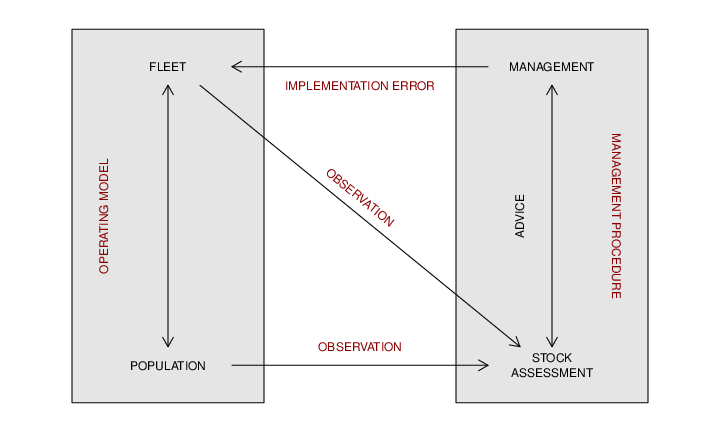
\includegraphics[height=0.8\textheight]{figs/mse.png}
\end{center}

\end{frame}

%*******************************************
\begin{frame}
\frametitle{Six steps to MSE\footnote{Punt, A. E., Butterworth, D. S., de, Moor, C. L., De Oliveira, J. A. and Haddon, M. (2016), Management strategy evaluation: best practices. Fish Fish, 17: 303-334. doi:10.1111/faf.12104}}

- Define and agree on objectives \& limits
- Identify appropriate Management Procedures
- Define a set of Operating Models
- Conduct simulations
- Summarize performance
- Select best MP

\end{frame}

%*******************************************
\begin{frame}
\frametitle{Define objectives \& limits}

- IOTC: target=$B_{MSY}$, limit=$0.40\cdot B_{MSY}$, also $P(Green) > 60\%$, over next 20
years.

\begin{center}
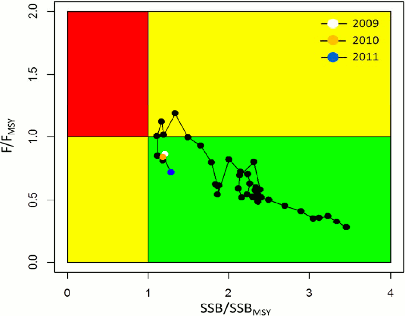
\includegraphics[height=0.4\textheight]{figs/kobe.png}
\end{center}

\begin{center}
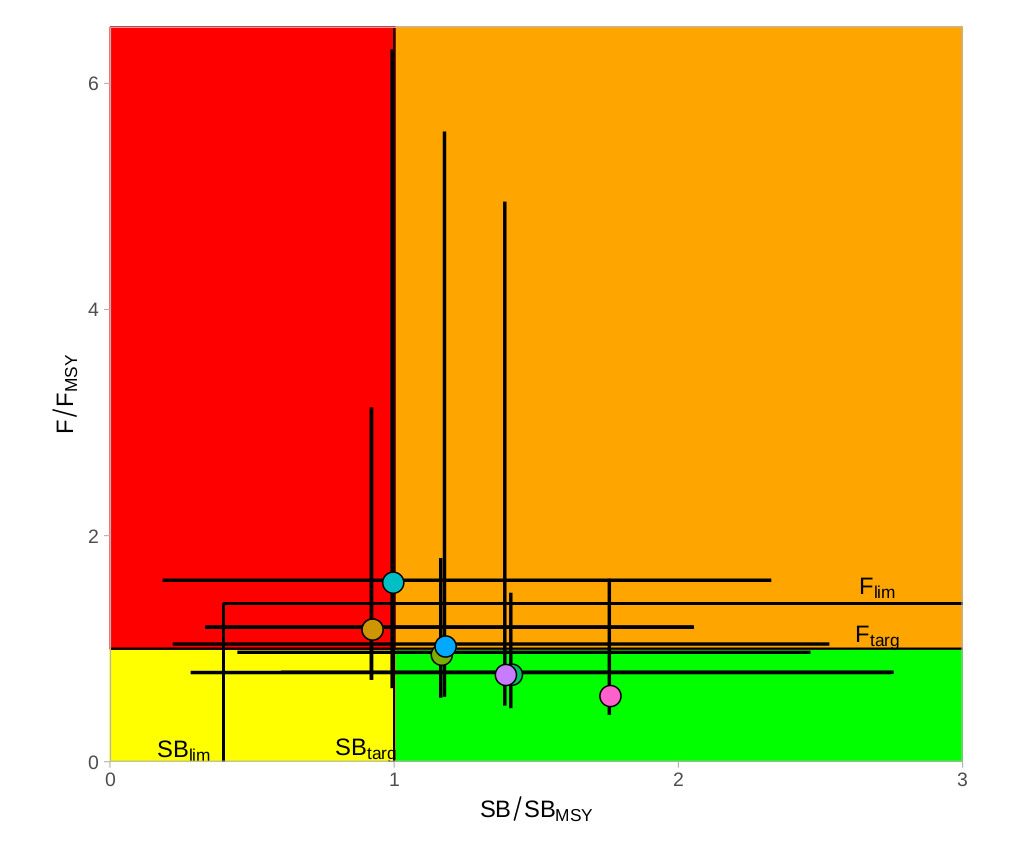
\includegraphics[height=0.4\textheight]{figs/kobe2.png}
\end{center}

\end{frame}

%*******************************************
\begin{frame}
\frametitle{Identify Management Procedures}

\begin{center}
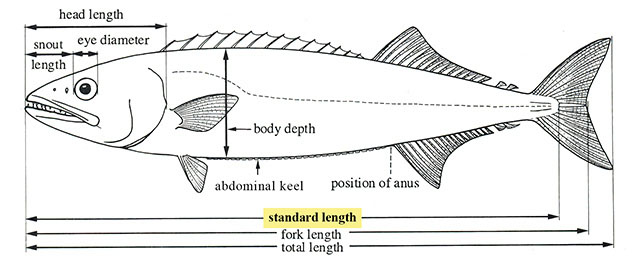
\includegraphics[height=0.18\textheight]{figs/sample}
\end{center}

\begin{center}

\includegraphics[height=0.25\textheight]{figs/ind.png}
\end{center}

\begin{center}
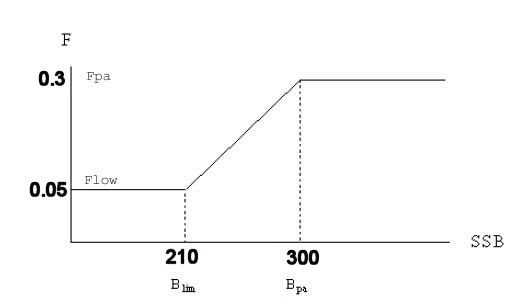
\includegraphics[height=0.25\textheight]{figs/hcr.png}
\end{center}

\end{frame}

%*******************************************
\begin{frame}
\frametitle{Define Operating Models}

\begin{center}
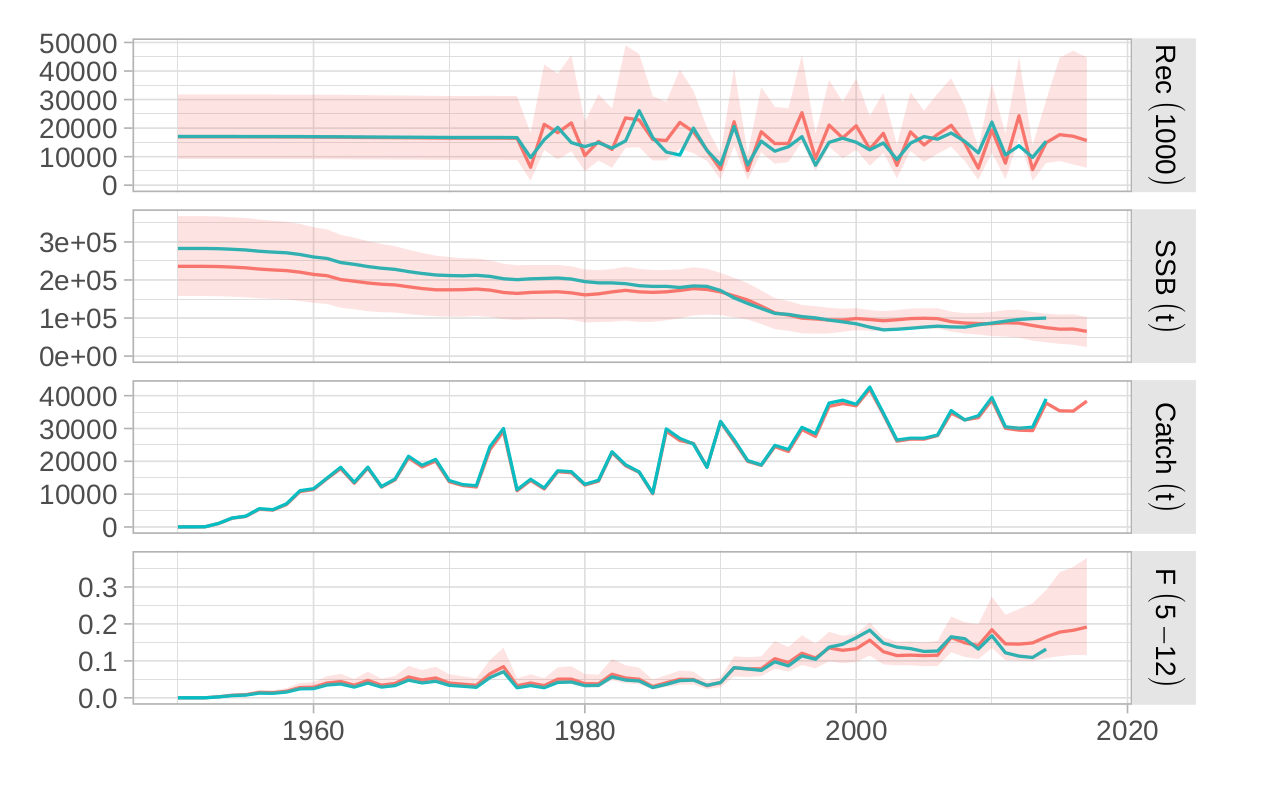
\includegraphics[height=0.95\textheight]{figs/om.png}
\end{center}

\end{frame}

%*******************************************
\begin{frame}
\frametitle{Conduct simulations}

\begin{center}
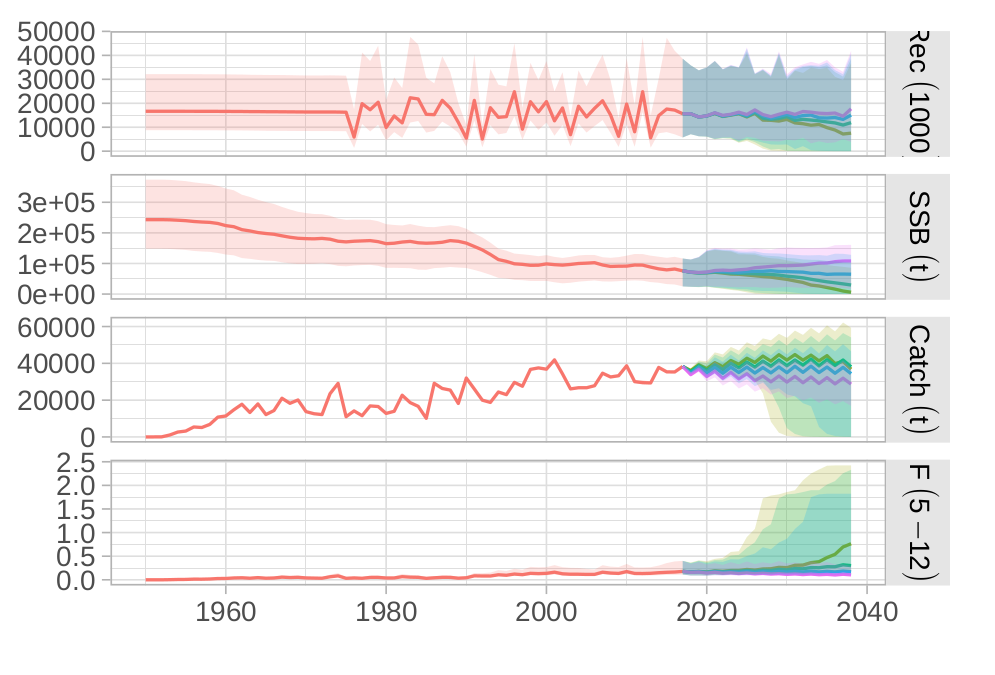
\includegraphics[height=0.95\textheight]{figs/runs.png}
\end{center}

\end{frame}

%*******************************************
\begin{frame}
\frametitle{Summarize performance}

\begin{center}
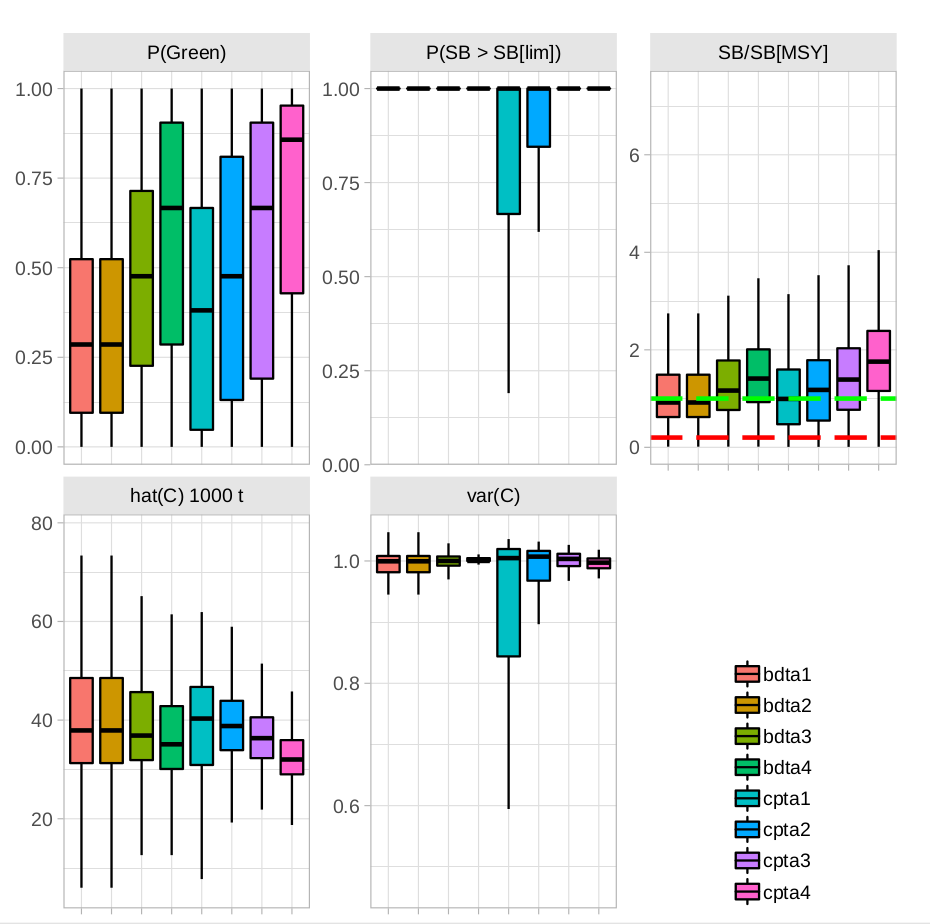
\includegraphics[height=0.5\textheight]{figs/perf1.png}
\end{center}

\begin{center}
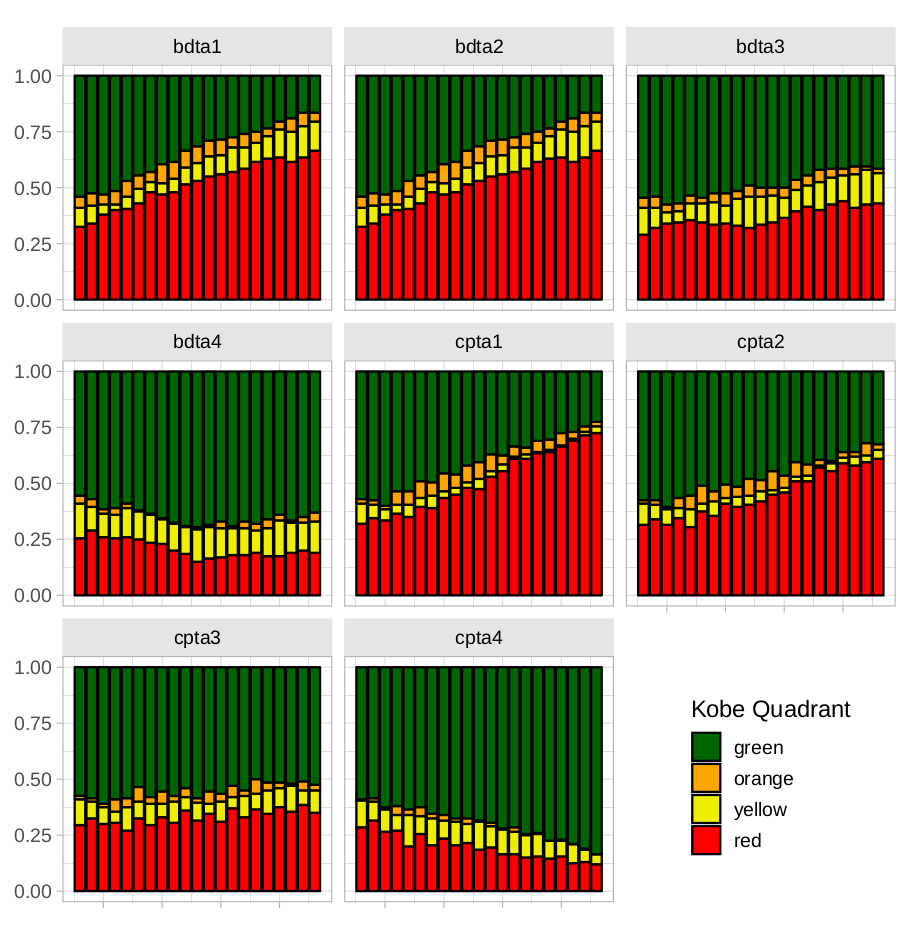
\includegraphics[height=0.5\textheight]{figs/perf2.png}
\end{center}

\end{frame}

%*******************************************
\begin{frame}
\frametitle{Select best MP}

\begin{center}
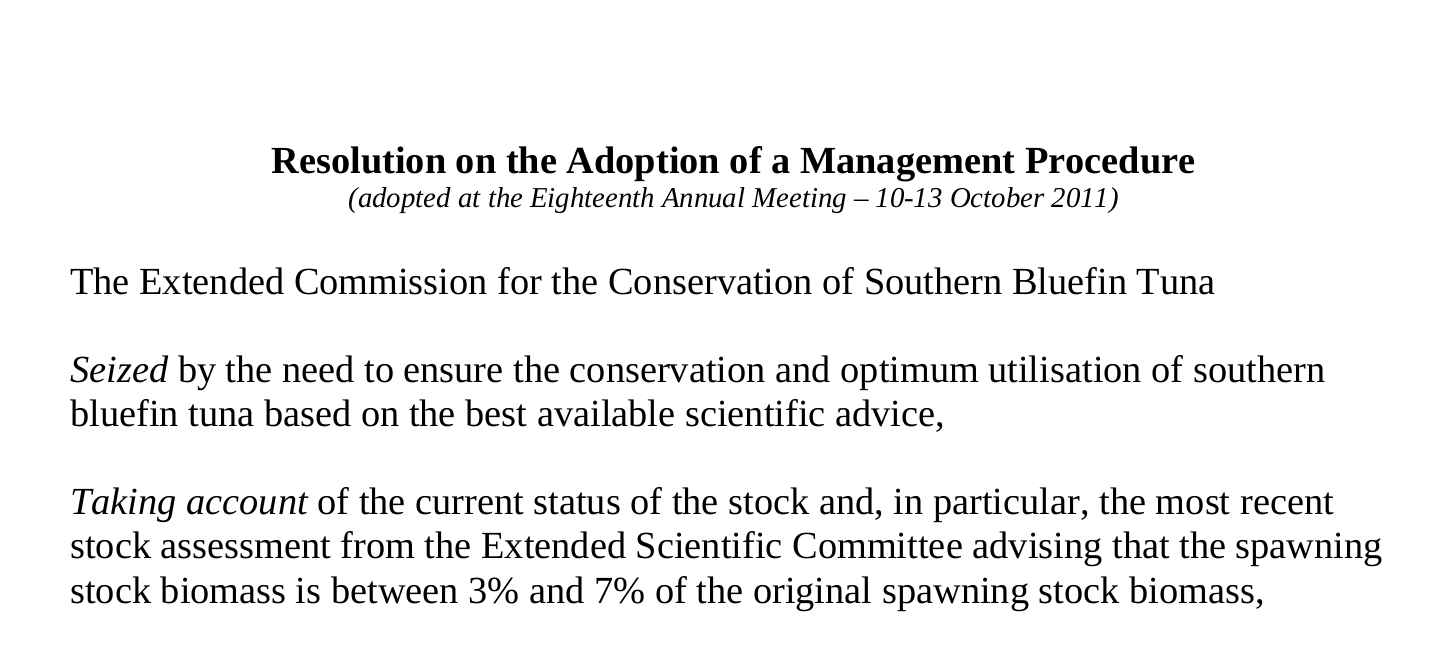
\includegraphics[height=0.95\textheight]{figs/mp.png}
\end{center}

\end{frame}

%*******************************************
\begin{frame}
\frametitle{What are the advantages?}

- Avoid being driven by yearly variability in SA
- Long-term trade-offs made clear
- Less haggling
- No wrong best assessment
- Default decision
- Risk on board
- Consistent with PA
- Interaction across the table

\end{frame}

%*******************************************
\begin{frame}
\frametitle{And disadvantages?}

- Results dependent on model (as usual)
- Lengthy development (less and less so)
- Data still essential (indeed)
- Overly rigid (up to you)
- Autopilot (exceptional circumstances)

\end{frame}
\end{document}
